\section{Results}

\subsection{General}
In the end we created a simulation of the solar system where you can see the planets move in real time. Since the planets are moving rather slowly in real time we have included a time skip function, meaning you can speed up the time to have the planets move around the sun in a noticeable pace, such that the motions of planets can be determined and is actually visible. The pace can be set to real time, ten times real time, one day per frame, or ten days per fram. A camera has been implemented to better allow for movement amongst the planets, allowing for visibility of orbital patterns even extending to Neptune, the planet furthest from the sun.
 
It clearly visible that the planets are moving around the sun according to the laws of gravity, and the theorem can be tested by the use of our comet cannon, which is capable of spawning comets as part of the system at the current camera position. Placing a comet sufficiently close to the sun or the other planets show distinct changes in orbital behaviour. The comets themselves follow the gravitational pull of the planets and change its trajectory accordingly, usually ending up orbiting the sun (the largest mass in the solar system).

\subsection{Textures}
\subsubsection{Custom UV coordinates}
All celestial objects are textured, yet the textures are warped and plagued with what I call the "Eye-of-Sauron" effect, see figure \ref{EyeOfSauron}. The Eye of Sauron effect is a result of texture stretching, and possibly a low polygon count on our object. The texture is stretched from one arc on the circle to the next, all the way around the textured object, except when it reaches the last arc, the texture is applied once more in full between the first and last arc.\\
This gives the spheres an odd look, where the texture is only applied to part of the figure, and not the figure in its entirety.\\
The Eye of Sauron effect is most likely a result of faulty math used in the GetTextureCoordinates() method (the CalcUVStretch method of SolarSimulation\_v2), which is a custom method used to derive UV-coordinates from XYZ-coordinates.
\begin{figure}
	\centering
	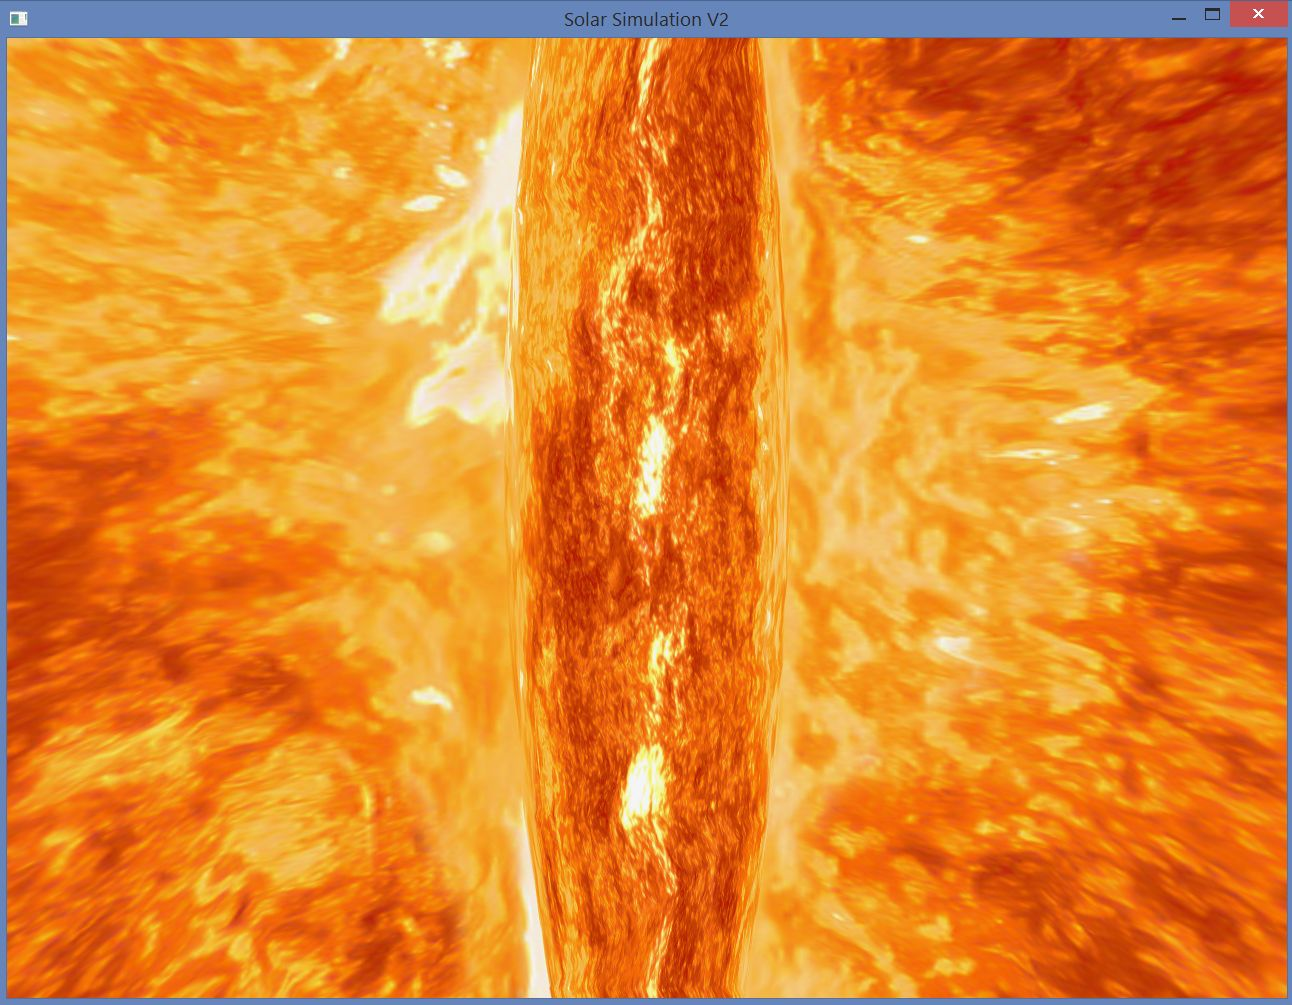
\includegraphics[scale=0.1]{Pictures/Bugs/EyeOfSauronEffectInitial}
	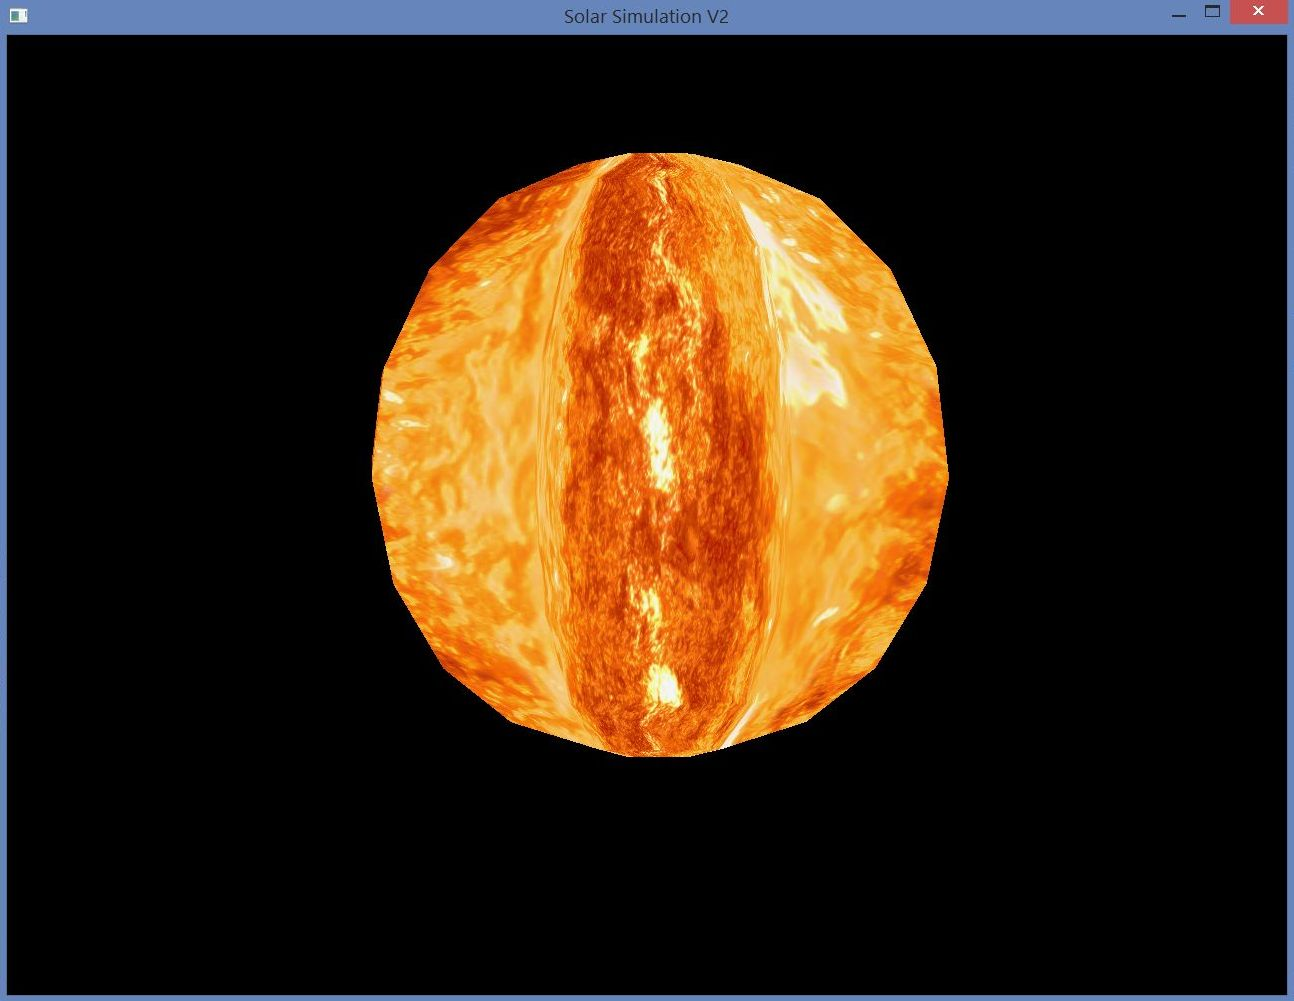
\includegraphics[scale=0.1]{Pictures/Bugs/EyeOfSauronEffectSun}
	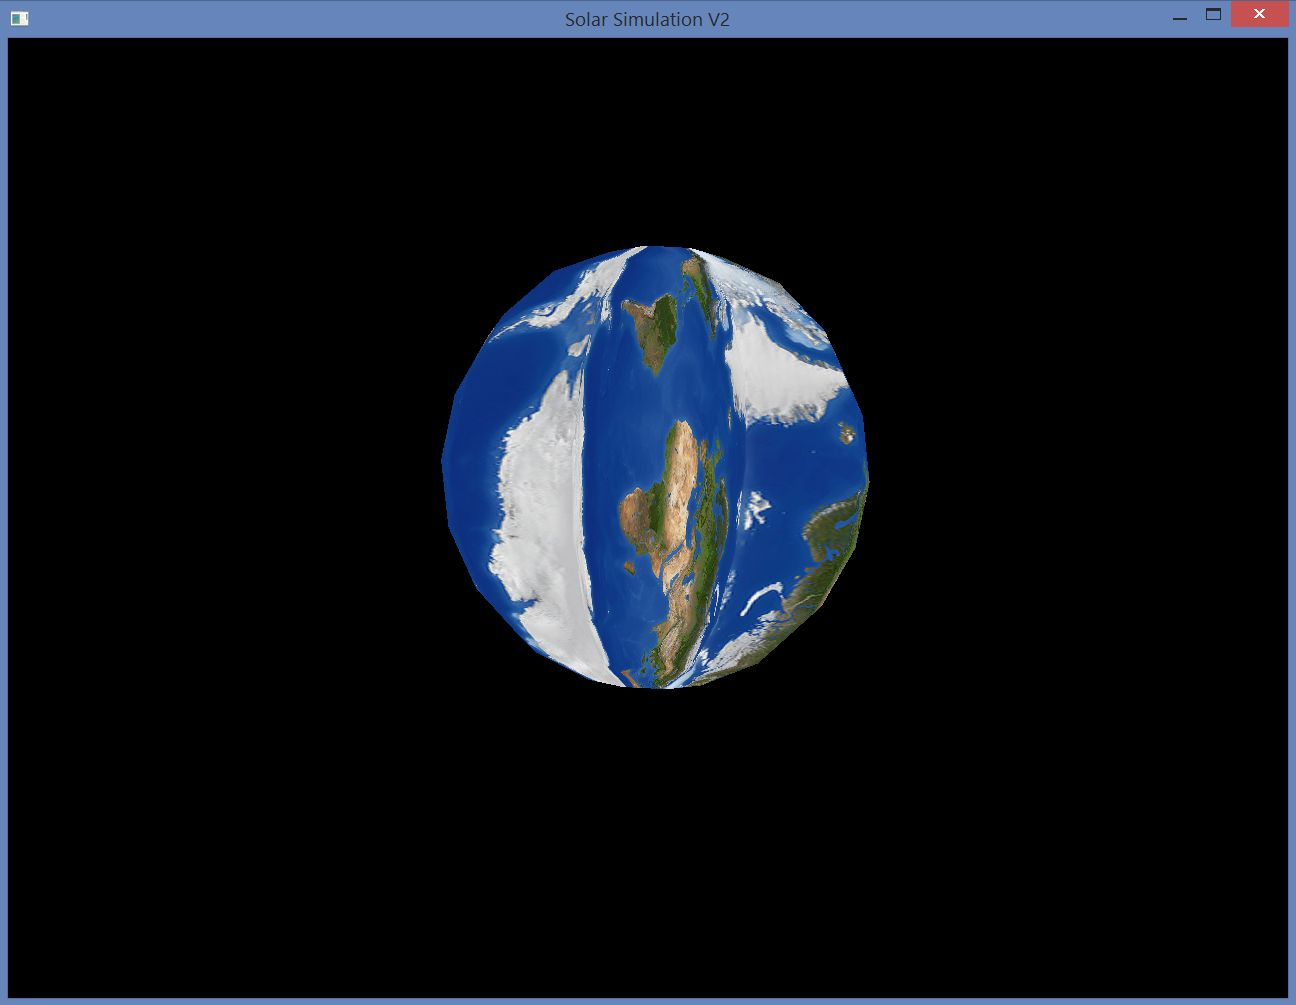
\includegraphics[scale=0.1]{Pictures/Bugs/EyeOfSauronEffectEarth}
	\label{EyeOfSauron}
	\caption{The Eye of Sauron effect. A result of bad texture stretching.}
\end{figure}
In addition to the Eye of Sauron effect, due to the vector calculatons within CalcUVStretch, the poles on each planet fails to render correctly. While stretching of the texture around the pole would be sufficient, the texture is instead discarded for the pole triangles, and the poles are largely painted with a single color, see figure \ref{PolarError}.\\
\begin{figure}
	\centering
	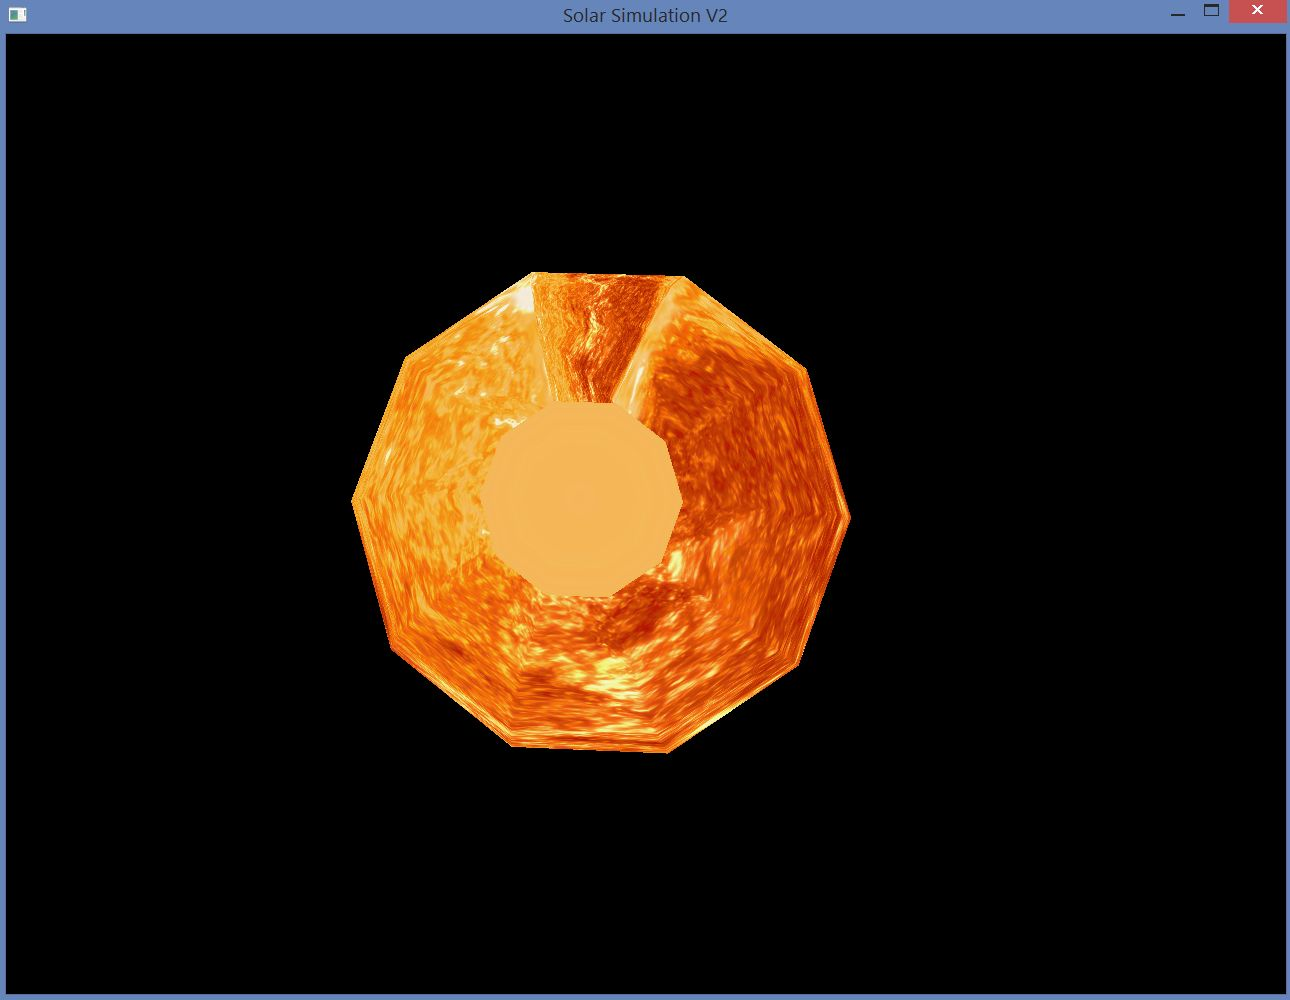
\includegraphics[scale=0.3]{Pictures/Bugs/PolarTextureError}
	\label{PolarError}
	\caption{The pole of the Sun painted with a single color, falsely derived from the texture.}
\end{figure}
To make matters even worse, the textures are not properly rotated on upon the figure, which is especially clear when looking at earth. Again, this seems to be a result of faulty math within the CalcUVStretch method.

\subsubsection{OpenTK TexGen - Quarter coverage of textures}
It is possible to have OpenTK generate UV-coordinates automatically when drawing vertices. This approach, while theoretically suitable and the easiest solution, leads to more interesting behaviour. In our case, the automatic coordinates cover only one quarter of the drawn object. This could be a consequence of the spheres having coordinates between -1 and 1, instead of 0 and 1, which is a requirement for precise UV-coordinate approximation by OpenTK.\\
Attempts to solve this has included serializing the spheres such that all coordinates were within 0 and 1, to no avail, yet due to the tight schedule of developement and the relative late attempt at solving the issue, this hypothesis has not been thoroughly tested.
\begin{figure}
	\centering
	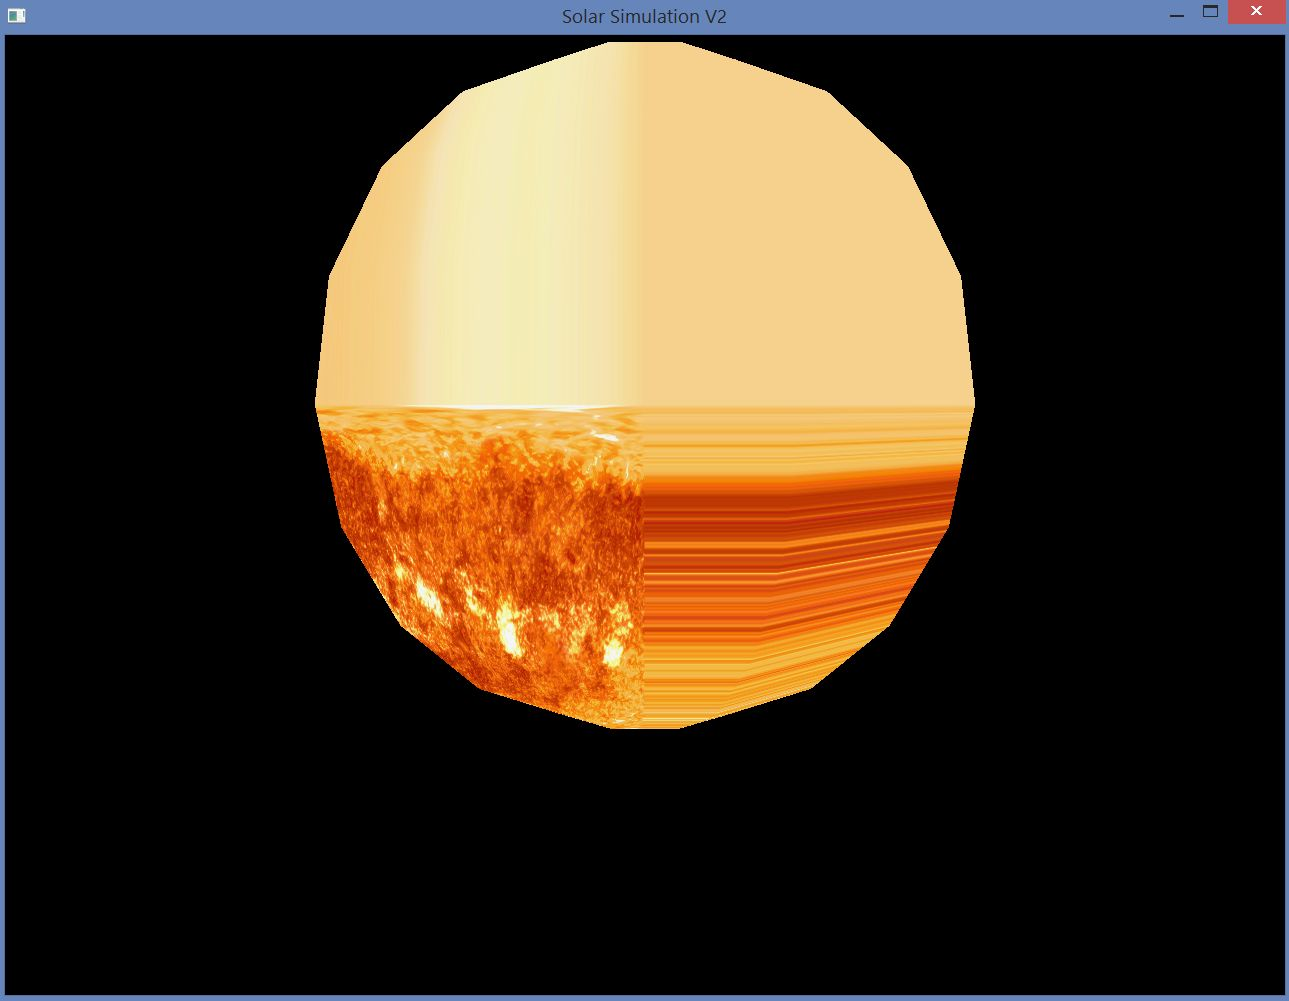
\includegraphics[scale=0.3]{Pictures/Bugs/TexGenQuarterCoverage}
	\label{TexGenError}
	\caption{Only one quarter of te total sphere is textured correctly, with the rest of the sphere being left with clamped textures.}
\end{figure}

\subsubsection{Clipping Errors}
When zooming along the Z-axis initially, an error in the face clipping becomes apparant. We have yet to identify the cause of this error, but the symptoms show that especially large objects suffer from this when the camera is sufficiently far away.\\
Within intervals, the front face of objects is clipped away, revealing multiple circles on the inside of the object. In addition, minor objects (such as the planets orbiting the sun) disappear in the same area, leaving us to believe that it is a bug in our viewing frustum.\\
With careful regulation of the zoom and positioning of the objects, the clipping error can be avoided, and it has no consequence regarding the physical attributes of the objects being rendered. Still, the error has only been identified by its symptoms, and efforts to track the cause has been fruitless.
\begin{figure}
	\centering
	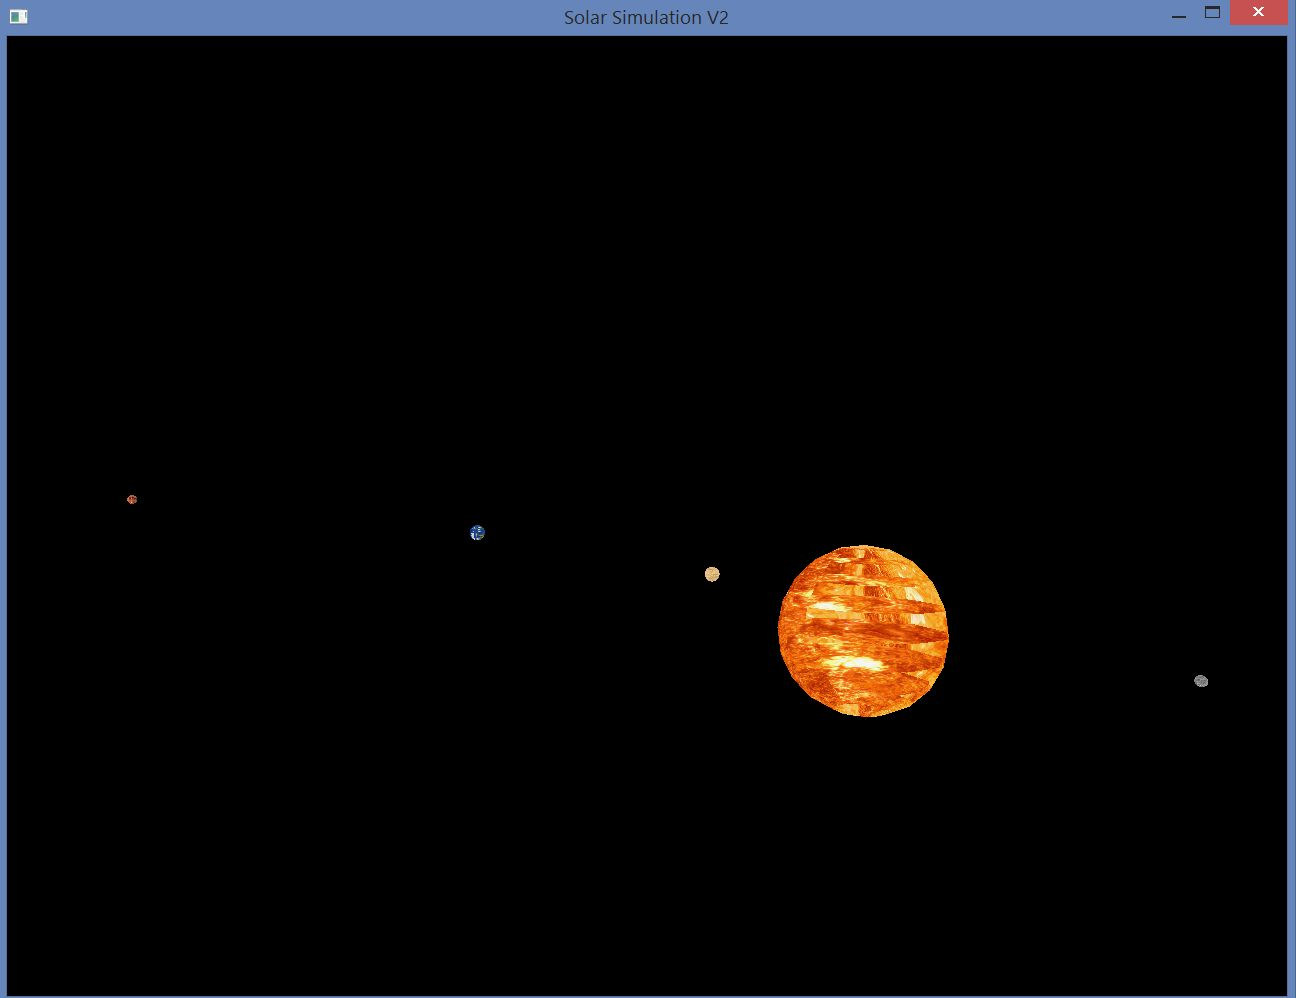
\includegraphics[scale=0.3]{Pictures/Bugs/ClippingError}
	\label{ClippingError}
	\caption{Within regular intervals, a clipping error appears, cutting out part of the view frustum. In this picture, the front face of the sun has been culled, which leads to errornous painting.}
\end{figure}